% =============================================================================
% Week 8: Linear Algebra I
% =============================================================================

\chapter{Week 8: Linear Algebra I}
\label{ch:week8}

\begin{bluebox}[Learning Objectives]
By the end of this week, you should be able to:
\begin{itemize}
    \item Define and distinguish between scalars, vectors, matrices, and tensors
    \item Use compact notation to express data structures in terms of real number spaces
    \item Perform matrix operations: transpose, addition, scalar multiplication, and matrix multiplication
    \item Verify conformability conditions for matrix multiplication
    \item Express systems of linear equations in matrix form
    \item Understand the identity matrix and its role in defining matrix inverses
    \item Compute and interpret vector norms ($L_1$, $L_2$, $L_\infty$)
    \item Derive the ordinary least squares (OLS) estimator using matrix calculus
    \item Understand and derive the Ridge, Lasso, and Elastic Net regression estimators
    \item Explain the geometric and statistical intuition behind regularisation
\end{itemize}
\end{bluebox}

\textbf{Prerequisites:} This week assumes familiarity with basic calculus (differentiation, partial derivatives), elementary algebra and equation manipulation, linear regression concepts from statistics courses, and summation notation.

% =============================================================================
\section{Data Structures in Linear Algebra}
\label{sec:data-structures}
% =============================================================================

Linear algebra provides the language and machinery for working with structured numerical data. Before diving into operations, we must understand the fundamental objects we manipulate.

\subsection{Scalars, Vectors, Matrices, and Tensors}

\begin{definition}[Scalar]
\label{def:scalar}
A \textbf{scalar} is a single numerical value. We denote scalars with lowercase letters:
\[
x = 5, \quad \alpha = 0.01, \quad c = -3.14
\]
Scalars are 0-dimensional objects---they have no notion of direction, only magnitude.
\end{definition}

\begin{definition}[Vector]
\label{def:vector}
A \textbf{vector} is an ordered list of scalars. We denote vectors with bold lowercase letters. By convention, vectors are \emph{column vectors}:
\[
\mathbf{x} = \begin{pmatrix} x_1 \\ x_2 \\ \vdots \\ x_n \end{pmatrix}
\]
A vector with $n$ elements is called an \textbf{$n$-dimensional vector} or an \textbf{$n$-vector}.
\end{definition}

\begin{intuition}[Geometric Interpretation of Vectors]
A vector can be visualised as an arrow in space:
\begin{itemize}
    \item A 2-dimensional vector $\mathbf{x} = \begin{pmatrix} 3 \\ 4 \end{pmatrix}$ represents an arrow from the origin to the point $(3, 4)$ in the plane.
    \item A 3-dimensional vector specifies a point (or direction) in 3D space.
    \item An $n$-dimensional vector specifies a point in $n$-dimensional space---harder to visualise but mathematically identical.
\end{itemize}
In data science, each element of a vector often represents a different feature or variable for a single observation.
\end{intuition}

\begin{definition}[Matrix]
\label{def:matrix}
A \textbf{matrix} is a rectangular array of scalars arranged in rows and columns. We denote matrices with bold uppercase letters:
\[
\mathbf{A} = \begin{pmatrix}
a_{11} & a_{12} & \cdots & a_{1n} \\
a_{21} & a_{22} & \cdots & a_{2n} \\
\vdots & \vdots & \ddots & \vdots \\
a_{m1} & a_{m2} & \cdots & a_{mn}
\end{pmatrix}
\]
This matrix has $m$ rows and $n$ columns, so we say it has dimensions $m \times n$ (read ``$m$ by $n$''). A generic element in row $i$ and column $j$ is denoted $a_{ij}$.
\end{definition}

\begin{warning}[Index Ordering Convention]
Matrix indices follow the convention [row, column], so $a_{ij}$ refers to row $i$, column $j$. This matches array indexing in languages like R and Julia, but note that Python uses 0-based indexing.

A common source of confusion: when we write dimensions as ``$m \times n$'', we mean $m$ rows and $n$ columns. The first number is always rows.
\end{warning}

In data science contexts:
\begin{itemize}
    \item Rows typically represent \textbf{observations} (data points, samples, individuals)
    \item Columns typically represent \textbf{variables} (features, attributes, predictors)
\end{itemize}
So a dataset with 100 observations and 5 features would be represented as a $100 \times 5$ matrix.

\begin{definition}[Tensor]
\label{def:tensor}
A \textbf{tensor} is a multi-dimensional array that generalises scalars, vectors, and matrices:
\begin{itemize}
    \item A scalar is a 0th-order tensor (0 indices needed)
    \item A vector is a 1st-order tensor (1 index needed: $x_i$)
    \item A matrix is a 2nd-order tensor (2 indices needed: $a_{ij}$)
    \item A 3rd-order tensor requires 3 indices: $a_{ijk}$
\end{itemize}
A 3rd-order tensor can be visualised as a cube or stack of matrices. Elements are indexed by three subscripts: $a_{ijk}$ refers to the element at position $(i, j, k)$.
\end{definition}

\begin{example}[Tensors in Practice]
\label{ex:tensors-practice}
Tensors appear naturally in many data science applications:
\begin{itemize}
    \item \textbf{Colour images:} A single RGB image is a 3rd-order tensor with dimensions (height $\times$ width $\times$ 3 colour channels).
    \item \textbf{Video:} A video is a 4th-order tensor (time $\times$ height $\times$ width $\times$ channels).
    \item \textbf{Batch processing:} In deep learning, a batch of images is a 4th-order tensor (batch size $\times$ height $\times$ width $\times$ channels).
\end{itemize}
\end{example}

\subsection{Compact Notation}

We use set membership notation to compactly express the type and dimensionality of mathematical objects.

\begin{bluebox}[Compact Notation for Data Structures]
\begin{align*}
\text{Scalar:} \quad & x \in \mathbb{R} \quad \text{(or equivalently } x \in \mathbb{R}^1\text{)} \\
\text{Vector:} \quad & \mathbf{x} \in \mathbb{R}^n \quad \text{($n$-dimensional column vector)} \\
\text{Matrix:} \quad & \mathbf{A} \in \mathbb{R}^{m \times n} \quad \text{($m$ rows, $n$ columns)} \\
\text{Tensor:} \quad & \mathbf{A} \in \mathbb{R}^{n_1 \times n_2 \times \cdots \times n_k} \quad \text{($k$th-order tensor)}
\end{align*}
The symbol $\mathbb{R}$ denotes the set of all real numbers. The notation $\mathbf{x} \in \mathbb{R}^n$ means ``$\mathbf{x}$ is an element of $n$-dimensional real space''---in other words, $\mathbf{x}$ is a vector of $n$ real numbers.
\end{bluebox}

\begin{remark}
\textbf{Row vs Column Vectors.} By convention, when we write $\mathbf{x} \in \mathbb{R}^n$ without further specification, we mean a column vector. To denote a row vector explicitly, we would write $\mathbf{x}^\top \in \mathbb{R}^{1 \times n}$ (a $1 \times n$ matrix).
\end{remark}

% =============================================================================
\section{The Transpose Operation}
\label{sec:transpose}
% =============================================================================

The transpose is one of the most fundamental matrix operations, interchanging rows and columns.

\begin{definition}[Transpose]
\label{def:transpose}
The \textbf{transpose} of a matrix $\mathbf{A} \in \mathbb{R}^{m \times n}$, denoted $\mathbf{A}^\top$ (or sometimes $\mathbf{A}'$), is the matrix $\mathbf{A}^\top \in \mathbb{R}^{n \times m}$ obtained by interchanging rows and columns:
\[
(\mathbf{A}^\top)_{ij} = a_{ji}
\]
That is, the element in row $i$, column $j$ of $\mathbf{A}^\top$ equals the element in row $j$, column $i$ of $\mathbf{A}$.
\end{definition}

\begin{example}[Transpose of a Matrix]
\label{ex:transpose-matrix}
\[
\mathbf{A} = \begin{pmatrix} a_{11} & a_{12} & a_{13} \\ a_{21} & a_{22} & a_{23} \end{pmatrix}
\quad \Longrightarrow \quad
\mathbf{A}^\top = \begin{pmatrix} a_{11} & a_{21} \\ a_{12} & a_{22} \\ a_{13} & a_{23} \end{pmatrix}
\]

With numerical values:
\[
\begin{pmatrix} 1 & 2 & 3 \\ 4 & 5 & 6 \end{pmatrix}^\top = \begin{pmatrix} 1 & 4 \\ 2 & 5 \\ 3 & 6 \end{pmatrix}
\]
\end{example}

\begin{intuition}[Visualising the Transpose]
Think of the transpose as flipping the matrix along its main diagonal (the diagonal from top-left to bottom-right). Equivalently:
\begin{enumerate}
    \item Take the first column of $\mathbf{A}$ and lay it out as the first row of $\mathbf{A}^\top$.
    \item Take the second column of $\mathbf{A}$ and lay it out as the second row of $\mathbf{A}^\top$.
    \item Continue for all columns.
\end{enumerate}
\end{intuition}

The transpose applies equally to vectors. Since vectors are column matrices:
\[
\mathbf{x} = \begin{pmatrix} x_1 \\ x_2 \\ x_3 \end{pmatrix}
\quad \Longrightarrow \quad
\mathbf{x}^\top = \begin{pmatrix} x_1 & x_2 & x_3 \end{pmatrix}
\]

A scalar can be viewed as a $1 \times 1$ matrix, so its transpose is itself.

\begin{theorem}[Properties of the Transpose]
\label{thm:transpose-properties}
For matrices $\mathbf{A}$ and $\mathbf{B}$ of appropriate dimensions, and scalar $c$:
\begin{align}
(\mathbf{A}^\top)^\top &= \mathbf{A} \label{eq:transpose-involution} \\
(\mathbf{A} + \mathbf{B})^\top &= \mathbf{A}^\top + \mathbf{B}^\top \label{eq:transpose-sum} \\
(c\mathbf{A})^\top &= c\mathbf{A}^\top \label{eq:transpose-scalar} \\
(\mathbf{A}\mathbf{B})^\top &= \mathbf{B}^\top \mathbf{A}^\top \label{eq:transpose-product}
\end{align}
\end{theorem}

\begin{warning}[Order Reversal in Products]
Equation~\eqref{eq:transpose-product} is crucial and frequently tested: the transpose of a product reverses the order of the factors. This extends to longer products:
\[
(\mathbf{A}\mathbf{B}\mathbf{C})^\top = \mathbf{C}^\top \mathbf{B}^\top \mathbf{A}^\top
\]
For vectors, this gives us: $(\mathbf{a}^\top \mathbf{b})^\top = \mathbf{b}^\top \mathbf{a}$. Since the dot product is a scalar, this tells us $\mathbf{a}^\top \mathbf{b} = \mathbf{b}^\top \mathbf{a}$---the dot product is commutative.
\end{warning}

\begin{definition}[Symmetric Matrix]
\label{def:symmetric-matrix}
A square matrix $\mathbf{A}$ is \textbf{symmetric} if $\mathbf{A}^\top = \mathbf{A}$, i.e., $a_{ij} = a_{ji}$ for all $i, j$.
\end{definition}

Symmetric matrices arise frequently in statistics and machine learning. For any matrix $\mathbf{X}$, the products $\mathbf{X}^\top \mathbf{X}$ and $\mathbf{X}\mathbf{X}^\top$ are always symmetric (verify this using the transpose properties).

% =============================================================================
\section{Matrix Addition and Scalar Multiplication}
\label{sec:matrix-add-scalar}
% =============================================================================

\subsection{Matrix Addition}

\begin{definition}[Matrix Addition]
\label{def:matrix-addition}
For two matrices $\mathbf{A}, \mathbf{B} \in \mathbb{R}^{m \times n}$ of identical dimensions, their sum $\mathbf{C} = \mathbf{A} + \mathbf{B}$ is defined element-wise:
\[
c_{ij} = a_{ij} + b_{ij} \quad \text{for all } i = 1, \ldots, m \text{ and } j = 1, \ldots, n
\]
\end{definition}

\begin{example}[Matrix Addition]
\label{ex:matrix-addition}
\[
\begin{pmatrix} 1 & 2 & 3 \\ 4 & 5 & 6 \end{pmatrix} + \begin{pmatrix} 1 & 2 & 1 \\ 1 & 1 & 0 \end{pmatrix} = \begin{pmatrix} 2 & 4 & 4 \\ 5 & 6 & 6 \end{pmatrix}
\]
\end{example}

\begin{warning}[Dimension Requirement]
Matrix addition is only defined when both matrices have exactly the same dimensions. You cannot add a $2 \times 3$ matrix to a $3 \times 2$ matrix---they must match in both rows and columns.
\end{warning}

\subsection{Scalar Multiplication}

\begin{definition}[Scalar Multiplication]
\label{def:scalar-multiplication}
For a scalar $c \in \mathbb{R}$ and matrix $\mathbf{A} \in \mathbb{R}^{m \times n}$, the product $c\mathbf{A}$ is defined element-wise:
\[
(c\mathbf{A})_{ij} = c \cdot a_{ij} \quad \text{for all } i, j
\]
\end{definition}

\begin{example}[Scalar Multiplication]
\label{ex:scalar-multiplication}
\[
3 \times \begin{pmatrix} 1 & 2 \\ 3 & 4 \end{pmatrix} = \begin{pmatrix} 3 & 6 \\ 9 & 12 \end{pmatrix}
\]
\end{example}

Scalar multiplication scales every element of the matrix by the same factor. Geometrically, for vectors, this stretches or shrinks the arrow (and reverses direction if the scalar is negative).

% =============================================================================
\section{Matrix Multiplication}
\label{sec:matrix-multiplication}
% =============================================================================

Matrix multiplication is perhaps the most important operation in linear algebra, but it is \emph{not} element-wise multiplication. Understanding this operation deeply is essential.

\subsection{The Dot Product (Inner Product)}

Before tackling general matrix multiplication, we start with the simpler case of multiplying two vectors.

\begin{definition}[Dot Product / Inner Product]
\label{def:dot-product}
For two vectors $\mathbf{a}, \mathbf{b} \in \mathbb{R}^n$ of equal length, their \textbf{dot product} (or \textbf{inner product}) is:
\[
\mathbf{a}^\top \mathbf{b} = \sum_{i=1}^{n} a_i b_i = a_1 b_1 + a_2 b_2 + \cdots + a_n b_n
\]
The result is a scalar.
\end{definition}

\begin{example}[Computing a Dot Product]
\label{ex:dot-product}
\[
\mathbf{a}^\top \mathbf{b} = \begin{pmatrix} 1 & 2 & 3 \end{pmatrix} \begin{pmatrix} 4 \\ 5 \\ 6 \end{pmatrix} = 1 \cdot 4 + 2 \cdot 5 + 3 \cdot 6 = 4 + 10 + 18 = 32
\]
\end{example}

\begin{intuition}[Geometric Interpretation of the Dot Product]
The dot product has a beautiful geometric interpretation. For vectors $\mathbf{a}$ and $\mathbf{b}$:
\[
\mathbf{a}^\top \mathbf{b} = \|\mathbf{a}\| \|\mathbf{b}\| \cos\theta
\]
where $\|\mathbf{a}\|$ and $\|\mathbf{b}\|$ are the lengths (norms) of the vectors and $\theta$ is the angle between them. This tells us:
\begin{itemize}
    \item \textbf{Positive dot product:} The vectors point in roughly the same direction ($\theta < 90^\circ$).
    \item \textbf{Zero dot product:} The vectors are orthogonal (perpendicular, $\theta = 90^\circ$).
    \item \textbf{Negative dot product:} The vectors point in roughly opposite directions ($\theta > 90^\circ$).
\end{itemize}
The dot product measures how much one vector points in the direction of another.
\end{intuition}

\subsection{Matrix-Matrix Multiplication}

\begin{definition}[Matrix Multiplication]
\label{def:matrix-multiplication}
For matrices $\mathbf{A} \in \mathbb{R}^{m \times n}$ and $\mathbf{B} \in \mathbb{R}^{n \times p}$, their product $\mathbf{C} = \mathbf{A}\mathbf{B}$ is a matrix $\mathbf{C} \in \mathbb{R}^{m \times p}$ where each element is:
\[
c_{ij} = \sum_{k=1}^{n} a_{ik} b_{kj} = a_{i1} b_{1j} + a_{i2} b_{2j} + \cdots + a_{in} b_{nj}
\]
Equivalently, $c_{ij}$ is the dot product of row $i$ of $\mathbf{A}$ with column $j$ of $\mathbf{B}$.
\end{definition}

\begin{bluebox}[Conformability and Output Dimensions]
\textbf{Conformability condition:} For $\mathbf{A}\mathbf{B}$ to be defined, the number of columns of $\mathbf{A}$ must equal the number of rows of $\mathbf{B}$.

\textbf{Mnemonic:} Think of the dimensions as $(m \times n) \cdot (n \times p) = (m \times p)$.
\begin{itemize}
    \item The \emph{inner dimensions} ($n$) must match---this is the conformability condition.
    \item The \emph{outer dimensions} ($m$ and $p$) give the shape of the result.
\end{itemize}
\end{bluebox}

\begin{example}[Matrix Multiplication: $2 \times 3$ by $3 \times 2$]
\label{ex:matrix-mult-2x3}
\[
\mathbf{A}\mathbf{B} = \begin{pmatrix} a_{11} & a_{12} & a_{13} \\ a_{21} & a_{22} & a_{23} \end{pmatrix} \begin{pmatrix} b_{11} & b_{12} \\ b_{21} & b_{22} \\ b_{31} & b_{32} \end{pmatrix} = \begin{pmatrix} a_{11}b_{11} + a_{12}b_{21} + a_{13}b_{31} & a_{11}b_{12} + a_{12}b_{22} + a_{13}b_{32} \\ a_{21}b_{11} + a_{22}b_{21} + a_{23}b_{31} & a_{21}b_{12} + a_{22}b_{22} + a_{23}b_{32} \end{pmatrix}
\]

Check: $(2 \times 3) \cdot (3 \times 2) = (2 \times 2)$. Inner dimensions match (both 3), output is $2 \times 2$.

Numerical example:
\[
\begin{pmatrix} 1 & 2 & 3 \\ 4 & 5 & 6 \end{pmatrix} \begin{pmatrix} 7 & 8 \\ 9 & 10 \\ 11 & 12 \end{pmatrix} = \begin{pmatrix} 1(7) + 2(9) + 3(11) & 1(8) + 2(10) + 3(12) \\ 4(7) + 5(9) + 6(11) & 4(8) + 5(10) + 6(12) \end{pmatrix} = \begin{pmatrix} 58 & 64 \\ 139 & 154 \end{pmatrix}
\]
\end{example}

\begin{rigour}[Algorithm for Matrix Multiplication]
To compute element $c_{ij}$ of the product $\mathbf{C} = \mathbf{A}\mathbf{B}$:
\begin{enumerate}
    \item Identify the $i$th row of $\mathbf{A}$: $(a_{i1}, a_{i2}, \ldots, a_{in})$
    \item Identify the $j$th column of $\mathbf{B}$: $(b_{1j}, b_{2j}, \ldots, b_{nj})^\top$
    \item Compute their dot product: $c_{ij} = \sum_{k=1}^{n} a_{ik} b_{kj}$
\end{enumerate}
Repeat for all $i \in \{1, \ldots, m\}$ and $j \in \{1, \ldots, p\}$.

\textbf{Visual heuristic:} To find $c_{ij}$, slide row $i$ of $\mathbf{A}$ across to column $j$ of $\mathbf{B}$, multiply corresponding elements, and sum.
\end{rigour}

\begin{bluebox}[Quick Reference: Small Matrix Products]
\textbf{$2 \times 2$ matrices:}
\[
\begin{pmatrix} a & b \\ c & d \end{pmatrix} \begin{pmatrix} e & f \\ g & h \end{pmatrix} = \begin{pmatrix} ae + bg & af + bh \\ ce + dg & cf + dh \end{pmatrix}
\]

\textbf{$3 \times 3$ matrices:}
\[
\begin{pmatrix} a & b & c \\ d & e & f \\ g & h & i \end{pmatrix} \begin{pmatrix} j & k & l \\ m & n & o \\ p & q & r \end{pmatrix} = \begin{pmatrix} aj + bm + cp & ak + bn + cq & al + bo + cr \\ dj + em + fp & dk + en + fq & dl + eo + fr \\ gj + hm + ip & gk + hn + iq & gl + ho + ir \end{pmatrix}
\]
\end{bluebox}

\begin{warning}[Matrix Multiplication is Not Commutative]
In general, $\mathbf{A}\mathbf{B} \neq \mathbf{B}\mathbf{A}$. In fact:
\begin{itemize}
    \item If $\mathbf{A}\mathbf{B}$ is defined, $\mathbf{B}\mathbf{A}$ might not even be defined (dimensions may not conform).
    \item Even when both products are defined, they may have different dimensions.
    \item Even when both products have the same dimensions, the matrices are typically different.
\end{itemize}
This non-commutativity is a major departure from scalar arithmetic and a common source of errors.
\end{warning}

\subsection{Matrix-Vector Multiplication}

Matrix-vector multiplication is a special case of matrix-matrix multiplication, but it is so common that it deserves explicit attention.

For $\mathbf{A} \in \mathbb{R}^{m \times n}$ and $\mathbf{x} \in \mathbb{R}^n$, the product $\mathbf{y} = \mathbf{A}\mathbf{x}$ is a vector $\mathbf{y} \in \mathbb{R}^m$ where:
\[
y_i = \sum_{j=1}^{n} a_{ij} x_j = a_{i1} x_1 + a_{i2} x_2 + \cdots + a_{in} x_n
\]

\begin{example}[Matrix-Vector Multiplication]
\label{ex:matrix-vector-mult}
\[
\begin{pmatrix} 1 & 2 & 3 \\ 4 & 5 & 6 \end{pmatrix} \begin{pmatrix} 7 \\ 8 \\ 9 \end{pmatrix} = \begin{pmatrix} 1(7) + 2(8) + 3(9) \\ 4(7) + 5(8) + 6(9) \end{pmatrix} = \begin{pmatrix} 50 \\ 122 \end{pmatrix}
\]

Check: $(2 \times 3) \cdot (3 \times 1) = (2 \times 1)$---the result is a 2-vector.
\end{example}

\begin{intuition}[Two Interpretations of $\mathbf{A}\mathbf{x}$]
There are two equivalent ways to think about matrix-vector multiplication:

\textbf{Row interpretation:} Each element of $\mathbf{y}$ is the dot product of a row of $\mathbf{A}$ with $\mathbf{x}$:
\[
y_i = (\text{row } i \text{ of } \mathbf{A}) \cdot \mathbf{x}
\]

\textbf{Column interpretation:} The result is a linear combination of the columns of $\mathbf{A}$, with coefficients given by $\mathbf{x}$:
\[
\mathbf{A}\mathbf{x} = x_1 \mathbf{a}_1 + x_2 \mathbf{a}_2 + \cdots + x_n \mathbf{a}_n
\]
where $\mathbf{a}_j$ is the $j$th column of $\mathbf{A}$.

The column interpretation is particularly important for understanding linear systems and the geometry of matrix transformations.
\end{intuition}

% =============================================================================
\section{Systems of Linear Equations}
\label{sec:linear-systems}
% =============================================================================

One of the most important applications of matrices is representing and solving systems of linear equations.

\subsection{Matrix Representation}

Consider a system of $m$ linear equations in $n$ unknowns:
\begin{align*}
a_{11} x_1 + a_{12} x_2 + \cdots + a_{1n} x_n &= b_1 \\
a_{21} x_1 + a_{22} x_2 + \cdots + a_{2n} x_n &= b_2 \\
&\vdots \\
a_{m1} x_1 + a_{m2} x_2 + \cdots + a_{mn} x_n &= b_m
\end{align*}

This system can be written compactly in matrix form as:
\begin{equation}
\mathbf{A}\mathbf{x} = \mathbf{b}
\label{eq:linear-system}
\end{equation}
where:
\[
\mathbf{A} = \begin{pmatrix}
a_{11} & a_{12} & \cdots & a_{1n} \\
a_{21} & a_{22} & \cdots & a_{2n} \\
\vdots & \vdots & \ddots & \vdots \\
a_{m1} & a_{m2} & \cdots & a_{mn}
\end{pmatrix}, \quad
\mathbf{x} = \begin{pmatrix} x_1 \\ x_2 \\ \vdots \\ x_n \end{pmatrix}, \quad
\mathbf{b} = \begin{pmatrix} b_1 \\ b_2 \\ \vdots \\ b_m \end{pmatrix}
\]

\begin{bluebox}[Components of a Linear System $\mathbf{A}\mathbf{x} = \mathbf{b}$]
\begin{itemize}
    \item $\mathbf{A} \in \mathbb{R}^{m \times n}$: The \textbf{coefficient matrix} containing the coefficients of the equations
    \item $\mathbf{x} \in \mathbb{R}^n$: The \textbf{unknown vector} we want to solve for
    \item $\mathbf{b} \in \mathbb{R}^m$: The \textbf{right-hand side vector} (constants)
\end{itemize}
In regression contexts: $\mathbf{A}$ is the design matrix (data), $\mathbf{x}$ is the coefficient vector, and $\mathbf{b}$ is the response vector.
\end{bluebox}

\subsection{Geometric Interpretation}

For a system of 2 equations in 2 unknowns, each equation represents a line in the plane. The solution is the intersection point. Three possibilities arise:
\begin{enumerate}
    \item \textbf{Unique solution:} The lines intersect at exactly one point.
    \item \textbf{No solution:} The lines are parallel (inconsistent system).
    \item \textbf{Infinitely many solutions:} The lines are identical (dependent system).
\end{enumerate}

In higher dimensions, each equation represents a hyperplane, and solutions are intersections of these hyperplanes.

\subsection{Gaussian Elimination}

Gaussian elimination is the standard algorithm for solving systems of linear equations. It systematically transforms the system into an equivalent one that is easier to solve.

\begin{definition}[Elementary Row Operations]
\label{def:elementary-row-ops}
The following operations on a matrix do not change the solution set of the corresponding linear system:
\begin{enumerate}
    \item \textbf{Row swap:} Interchange two rows ($R_i \leftrightarrow R_j$).
    \item \textbf{Row scaling:} Multiply a row by a non-zero constant ($R_i \to c \cdot R_i$, $c \neq 0$).
    \item \textbf{Row addition:} Add a multiple of one row to another ($R_i \to R_i + c \cdot R_j$).
\end{enumerate}
\end{definition}

\begin{definition}[Augmented Matrix]
\label{def:augmented-matrix}
The \textbf{augmented matrix} $[\mathbf{A} \mid \mathbf{b}]$ combines the coefficient matrix and right-hand side:
\[
[\mathbf{A} \mid \mathbf{b}] = \left(\begin{array}{cccc|c}
a_{11} & a_{12} & \cdots & a_{1n} & b_1 \\
a_{21} & a_{22} & \cdots & a_{2n} & b_2 \\
\vdots & \vdots & \ddots & \vdots & \vdots \\
a_{m1} & a_{m2} & \cdots & a_{mn} & b_m
\end{array}\right)
\]
\end{definition}

\begin{rigour}[Gaussian Elimination Algorithm]
\textbf{Goal:} Transform the augmented matrix to row echelon form (REF), where:
\begin{itemize}
    \item All rows consisting entirely of zeros are at the bottom.
    \item The leading entry (pivot) of each non-zero row is to the right of the pivot in the row above.
    \item All entries below each pivot are zero.
\end{itemize}

\textbf{Forward elimination (achieving REF):}
\begin{enumerate}
    \item Start with column 1. Find the first non-zero entry (pivot). If needed, swap rows to bring it to position (1,1).
    \item Use row operations to eliminate all entries below the pivot.
    \item Move to column 2, row 2. Repeat: find pivot, eliminate entries below.
    \item Continue until the matrix is in REF.
\end{enumerate}

\textbf{Back substitution:} Starting from the last equation, solve for each variable and substitute back into earlier equations.

For reduced row echelon form (RREF), continue with:
\begin{enumerate}
    \item Scale each pivot to 1.
    \item Use row operations to eliminate all entries above each pivot as well.
\end{enumerate}
\end{rigour}

\begin{example}[Gaussian Elimination]
\label{ex:gaussian-elimination}
Solve the system:
\begin{align*}
x + 2y + z &= 9 \\
2x + 4y + 3z &= 21 \\
3x + 5y + 4z &= 25
\end{align*}

\textbf{Step 1:} Form the augmented matrix.
\[
\left(\begin{array}{ccc|c}
1 & 2 & 1 & 9 \\
2 & 4 & 3 & 21 \\
3 & 5 & 4 & 25
\end{array}\right)
\]

\textbf{Step 2:} Eliminate entries below pivot in column 1.
\[
R_2 \to R_2 - 2R_1: \quad \left(\begin{array}{ccc|c}
1 & 2 & 1 & 9 \\
0 & 0 & 1 & 3 \\
3 & 5 & 4 & 25
\end{array}\right)
\]
\[
R_3 \to R_3 - 3R_1: \quad \left(\begin{array}{ccc|c}
1 & 2 & 1 & 9 \\
0 & 0 & 1 & 3 \\
0 & -1 & 1 & -2
\end{array}\right)
\]

\textbf{Step 3:} Swap $R_2$ and $R_3$ to get a pivot in position (2,2).
\[
\left(\begin{array}{ccc|c}
1 & 2 & 1 & 9 \\
0 & -1 & 1 & -2 \\
0 & 0 & 1 & 3
\end{array}\right)
\]

\textbf{Step 4:} Back substitution.
\begin{itemize}
    \item From row 3: $z = 3$
    \item From row 2: $-y + z = -2 \Rightarrow -y + 3 = -2 \Rightarrow y = 5$
    \item From row 1: $x + 2y + z = 9 \Rightarrow x + 10 + 3 = 9 \Rightarrow x = -4$
\end{itemize}

\textbf{Solution:} $(x, y, z) = (-4, 5, 3)$.
\end{example}

% =============================================================================
\section{The Identity Matrix and Matrix Inverses}
\label{sec:identity-inverse}
% =============================================================================

\subsection{The Identity Matrix}

\begin{definition}[Identity Matrix]
\label{def:identity-matrix}
The \textbf{identity matrix} $\mathbf{I}_n$ is the $n \times n$ square matrix with 1s on the main diagonal and 0s elsewhere:
\[
\mathbf{I}_n = \begin{pmatrix}
1 & 0 & \cdots & 0 \\
0 & 1 & \cdots & 0 \\
\vdots & \vdots & \ddots & \vdots \\
0 & 0 & \cdots & 1
\end{pmatrix}
\]

For example:
\[
\mathbf{I}_2 = \begin{pmatrix} 1 & 0 \\ 0 & 1 \end{pmatrix}, \quad
\mathbf{I}_3 = \begin{pmatrix} 1 & 0 & 0 \\ 0 & 1 & 0 \\ 0 & 0 & 1 \end{pmatrix}
\]
\end{definition}

The identity matrix is the matrix analogue of the number 1 in scalar arithmetic. It is the \textbf{multiplicative identity}.

\begin{theorem}[Properties of the Identity Matrix]
\label{thm:identity-properties}
For any matrix $\mathbf{A} \in \mathbb{R}^{m \times n}$:
\begin{align}
\mathbf{I}_m \mathbf{A} &= \mathbf{A} \label{eq:identity-left} \\
\mathbf{A} \mathbf{I}_n &= \mathbf{A} \label{eq:identity-right}
\end{align}
For any vector $\mathbf{x} \in \mathbb{R}^n$:
\[
\mathbf{I}_n \mathbf{x} = \mathbf{x}
\]
Multiplying by the identity matrix does nothing---it returns the original matrix or vector unchanged.
\end{theorem}

\subsection{The Matrix Inverse}

\begin{definition}[Matrix Inverse]
\label{def:matrix-inverse}
For a square matrix $\mathbf{A} \in \mathbb{R}^{n \times n}$, if there exists a matrix $\mathbf{A}^{-1}$ such that:
\[
\mathbf{A}^{-1} \mathbf{A} = \mathbf{A} \mathbf{A}^{-1} = \mathbf{I}_n
\]
then $\mathbf{A}^{-1}$ is called the \textbf{inverse} of $\mathbf{A}$, and $\mathbf{A}$ is said to be \textbf{invertible} (or \textbf{non-singular}).
\end{definition}

\begin{warning}[Existence of the Inverse]
\begin{itemize}
    \item \textbf{Only square matrices can have inverses.} A $3 \times 4$ matrix cannot be inverted.
    \item \textbf{Not all square matrices have inverses.} A matrix without an inverse is called \emph{singular} or \emph{non-invertible}.
    \item A square matrix is invertible if and only if its determinant is non-zero (equivalently, if its columns/rows are linearly independent---see \cref{ch:week9}).
\end{itemize}
\end{warning}

The inverse is theoretically important for solving linear systems. If $\mathbf{A}\mathbf{x} = \mathbf{b}$ and $\mathbf{A}$ is invertible:
\[
\mathbf{x} = \mathbf{A}^{-1} \mathbf{b}
\]

However, in practice, directly computing $\mathbf{A}^{-1}$ is often avoided because it is computationally expensive and numerically unstable. Instead, we use algorithms like Gaussian elimination or matrix factorisations.

\begin{theorem}[Properties of the Inverse]
\label{thm:inverse-properties}
For invertible matrices $\mathbf{A}$ and $\mathbf{B}$ of compatible dimensions:
\begin{align}
(\mathbf{A}^{-1})^{-1} &= \mathbf{A} \label{eq:inverse-involution} \\
(\mathbf{A}^\top)^{-1} &= (\mathbf{A}^{-1})^\top \label{eq:inverse-transpose} \\
(\mathbf{A}\mathbf{B})^{-1} &= \mathbf{B}^{-1} \mathbf{A}^{-1} \quad \text{(order reverses)} \label{eq:inverse-product}
\end{align}
\end{theorem}

% =============================================================================
\section{Vector Norms}
\label{sec:vector-norms}
% =============================================================================

Norms provide a way to measure the ``size'' or ``length'' of vectors. Different norms emphasise different aspects of a vector.

\begin{definition}[Vector Norm]
\label{def:vector-norm}
A \textbf{norm} on $\mathbb{R}^n$ is a function $\|\cdot\| : \mathbb{R}^n \to \mathbb{R}$ satisfying:
\begin{enumerate}
    \item \textbf{Non-negativity:} $\|\mathbf{x}\| \geq 0$, with equality if and only if $\mathbf{x} = \mathbf{0}$.
    \item \textbf{Absolute homogeneity:} $\|c\mathbf{x}\| = |c| \|\mathbf{x}\|$ for any scalar $c$.
    \item \textbf{Triangle inequality:} $\|\mathbf{x} + \mathbf{y}\| \leq \|\mathbf{x}\| + \|\mathbf{y}\|$.
\end{enumerate}
\end{definition}

\begin{bluebox}[Common Vector Norms]
For $\mathbf{x} = (x_1, x_2, \ldots, x_n)^\top \in \mathbb{R}^n$:

\textbf{$L_1$ norm (Manhattan / Taxicab norm):}
\[
\|\mathbf{x}\|_1 = \sum_{i=1}^{n} |x_i| = |x_1| + |x_2| + \cdots + |x_n|
\]

\textbf{$L_2$ norm (Euclidean norm):}
\[
\|\mathbf{x}\|_2 = \sqrt{\sum_{i=1}^{n} x_i^2} = \sqrt{x_1^2 + x_2^2 + \cdots + x_n^2}
\]

\textbf{$L_\infty$ norm (Maximum / Chebyshev norm):}
\[
\|\mathbf{x}\|_\infty = \max_i |x_i|
\]
\end{bluebox}

\begin{intuition}[Geometric Interpretation of Norms]
Consider the set of all vectors with norm equal to 1 (the \emph{unit ball}). The shape of this set differs by norm:
\begin{itemize}
    \item \textbf{$L_2$ norm:} The unit ball is a circle (2D) or sphere (3D)---all points at Euclidean distance 1 from the origin.
    \item \textbf{$L_1$ norm:} The unit ball is a diamond (2D) or octahedron (3D). The $L_1$ distance is like navigating a city grid where you can only move along axes (hence ``taxicab'' or ``Manhattan'' distance).
    \item \textbf{$L_\infty$ norm:} The unit ball is a square (2D) or cube (3D). The norm equals the largest coordinate in absolute value.
\end{itemize}

\begin{center}
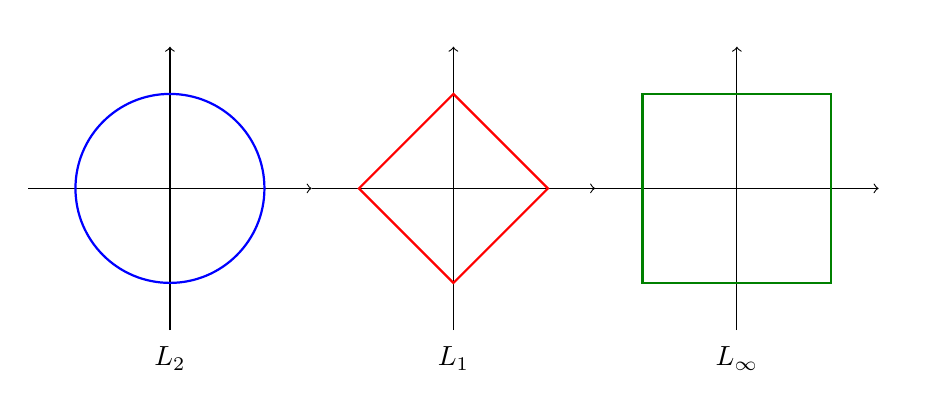
\begin{tikzpicture}[scale=1.2]
% L2 norm (circle)
\begin{scope}[shift={(-3,0)}]
\draw[->] (-1.5,0) -- (1.5,0) node[right] {};
\draw[->] (0,-1.5) -- (0,1.5) node[above] {};
\draw[thick, blue] (0,0) circle (1);
\node at (0,-1.8) {$L_2$};
\end{scope}

% L1 norm (diamond)
\begin{scope}
\draw[->] (-1.5,0) -- (1.5,0) node[right] {};
\draw[->] (0,-1.5) -- (0,1.5) node[above] {};
\draw[thick, red] (1,0) -- (0,1) -- (-1,0) -- (0,-1) -- cycle;
\node at (0,-1.8) {$L_1$};
\end{scope}

% L_infty norm (square)
\begin{scope}[shift={(3,0)}]
\draw[->] (-1.5,0) -- (1.5,0) node[right] {};
\draw[->] (0,-1.5) -- (0,1.5) node[above] {};
\draw[thick, green!50!black] (-1,-1) rectangle (1,1);
\node at (0,-1.8) {$L_\infty$};
\end{scope}
\end{tikzpicture}
\end{center}
\end{intuition}

\begin{example}[Computing Norms]
\label{ex:computing-norms}
For $\mathbf{x} = \begin{pmatrix} 3 \\ -4 \end{pmatrix}$:
\begin{align*}
\|\mathbf{x}\|_1 &= |3| + |-4| = 7 \\
\|\mathbf{x}\|_2 &= \sqrt{3^2 + (-4)^2} = \sqrt{9 + 16} = 5 \\
\|\mathbf{x}\|_\infty &= \max(|3|, |-4|) = 4
\end{align*}
Note that the $L_2$ norm of $(3, -4)$ equals 5---this is the familiar 3-4-5 right triangle from the Pythagorean theorem.
\end{example}

The choice of norm matters significantly in applications like regularisation (see \cref{sec:penalised-regression}) and optimisation.

% =============================================================================
\section{Linear Regression in Matrix Form}
\label{sec:linear-regression-matrix}
% =============================================================================

Linear regression is one of the most important applications of linear algebra in data science. We now derive the ordinary least squares (OLS) estimator using matrix calculus.

\subsection{The Linear Model}

For $n$ observations, each with $p$ predictor variables, the linear regression model assumes:
\begin{equation}
y_i = \beta_0 + \beta_1 x_{i1} + \beta_2 x_{i2} + \cdots + \beta_p x_{ip} + \varepsilon_i, \quad i = 1, \ldots, n
\label{eq:linear-model-scalar}
\end{equation}
where $y_i$ is the response for observation $i$, the $x_{ij}$ are predictor values, the $\beta_j$ are unknown coefficients, and $\varepsilon_i$ is the error term.

\begin{bluebox}[Matrix Form of Linear Regression]
We can write the entire system compactly as:
\begin{equation}
\mathbf{y} = \mathbf{X}\boldsymbol{\beta} + \boldsymbol{\varepsilon}
\label{eq:linear-model-matrix}
\end{equation}
where:
\[
\mathbf{y} = \begin{pmatrix} y_1 \\ y_2 \\ \vdots \\ y_n \end{pmatrix}, \quad
\mathbf{X} = \begin{pmatrix}
1 & x_{11} & x_{12} & \cdots & x_{1p} \\
1 & x_{21} & x_{22} & \cdots & x_{2p} \\
\vdots & \vdots & \vdots & \ddots & \vdots \\
1 & x_{n1} & x_{n2} & \cdots & x_{np}
\end{pmatrix}, \quad
\boldsymbol{\beta} = \begin{pmatrix} \beta_0 \\ \beta_1 \\ \vdots \\ \beta_p \end{pmatrix}, \quad
\boldsymbol{\varepsilon} = \begin{pmatrix} \varepsilon_1 \\ \varepsilon_2 \\ \vdots \\ \varepsilon_n \end{pmatrix}
\]

\textbf{Dimensions:}
\begin{itemize}
    \item $\mathbf{y} \in \mathbb{R}^n$: Response vector
    \item $\mathbf{X} \in \mathbb{R}^{n \times (p+1)}$: Design matrix (the column of 1s handles the intercept)
    \item $\boldsymbol{\beta} \in \mathbb{R}^{p+1}$: Coefficient vector
    \item $\boldsymbol{\varepsilon} \in \mathbb{R}^n$: Error vector
\end{itemize}
\end{bluebox}

\begin{remark}
\textbf{Why the Column of Ones?} The first column of $\mathbf{X}$ consists entirely of 1s. When multiplied by $\beta_0$, this produces the constant intercept term in each equation. This trick allows us to treat the intercept uniformly with the other coefficients.
\end{remark}

\subsection{The Least Squares Objective}

Our goal is to find the coefficient vector $\boldsymbol{\beta}$ that minimises the sum of squared errors (residuals):
\begin{equation}
\text{SSE} = \sum_{i=1}^{n} \varepsilon_i^2 = \sum_{i=1}^{n} (y_i - \hat{y}_i)^2
\label{eq:sse-scalar}
\end{equation}
where $\hat{y}_i = \beta_0 + \beta_1 x_{i1} + \cdots + \beta_p x_{ip}$ is the predicted value.

In matrix notation, the sum of squared errors can be written elegantly:
\begin{equation}
\text{SSE} = \boldsymbol{\varepsilon}^\top \boldsymbol{\varepsilon} = (\mathbf{y} - \mathbf{X}\boldsymbol{\beta})^\top (\mathbf{y} - \mathbf{X}\boldsymbol{\beta})
\label{eq:sse-matrix}
\end{equation}

\begin{rigour}[Equivalence of Scalar and Matrix SSE]
To see why $\sum_i \varepsilon_i^2 = \boldsymbol{\varepsilon}^\top \boldsymbol{\varepsilon}$, note that:
\[
\boldsymbol{\varepsilon}^\top \boldsymbol{\varepsilon} = \begin{pmatrix} \varepsilon_1 & \varepsilon_2 & \cdots & \varepsilon_n \end{pmatrix} \begin{pmatrix} \varepsilon_1 \\ \varepsilon_2 \\ \vdots \\ \varepsilon_n \end{pmatrix} = \varepsilon_1^2 + \varepsilon_2^2 + \cdots + \varepsilon_n^2 = \sum_{i=1}^{n} \varepsilon_i^2
\]
This is the dot product of $\boldsymbol{\varepsilon}$ with itself, which equals the sum of squared elements.
\end{rigour}

\subsection{Expanding the Objective Function}

To find the minimum, we need to expand the objective function and take its derivative. Let us expand $(\mathbf{y} - \mathbf{X}\boldsymbol{\beta})^\top (\mathbf{y} - \mathbf{X}\boldsymbol{\beta})$.

\begin{rigour}[Expansion of the SSE]
Using the transpose properties from \cref{thm:transpose-properties}:
\begin{align*}
\text{SSE} &= (\mathbf{y} - \mathbf{X}\boldsymbol{\beta})^\top (\mathbf{y} - \mathbf{X}\boldsymbol{\beta}) \\
&= \mathbf{y}^\top \mathbf{y} - \mathbf{y}^\top \mathbf{X}\boldsymbol{\beta} - (\mathbf{X}\boldsymbol{\beta})^\top \mathbf{y} + (\mathbf{X}\boldsymbol{\beta})^\top (\mathbf{X}\boldsymbol{\beta})
\end{align*}

For the cross terms, note that:
\begin{itemize}
    \item $(\mathbf{X}\boldsymbol{\beta})^\top = \boldsymbol{\beta}^\top \mathbf{X}^\top$ (transpose of a product reverses order)
    \item $\mathbf{y}^\top \mathbf{X}\boldsymbol{\beta}$ is a scalar, and the transpose of a scalar is itself
    \item Therefore $\mathbf{y}^\top \mathbf{X}\boldsymbol{\beta} = (\mathbf{y}^\top \mathbf{X}\boldsymbol{\beta})^\top = \boldsymbol{\beta}^\top \mathbf{X}^\top \mathbf{y}$
\end{itemize}

So both cross terms are equal, and:
\begin{equation}
\text{SSE} = \mathbf{y}^\top \mathbf{y} - 2\boldsymbol{\beta}^\top \mathbf{X}^\top \mathbf{y} + \boldsymbol{\beta}^\top \mathbf{X}^\top \mathbf{X}\boldsymbol{\beta}
\label{eq:sse-expanded}
\end{equation}
Equivalently: $\text{SSE} = \mathbf{y}^\top \mathbf{y} - \mathbf{y}^\top \mathbf{X}\boldsymbol{\beta} - \boldsymbol{\beta}^\top \mathbf{X}^\top \mathbf{y} + \boldsymbol{\beta}^\top \mathbf{X}^\top \mathbf{X}\boldsymbol{\beta}$
\end{rigour}

\subsection{Deriving the OLS Estimator}

To minimise SSE, we differentiate with respect to $\boldsymbol{\beta}$ and set the derivative equal to zero.

\begin{bluebox}[Matrix Calculus: Key Results]
We need two results from matrix calculus (see the Matrix Cookbook for comprehensive reference):

For a vector $\mathbf{a}$ and matrices of appropriate dimensions:
\begin{enumerate}
    \item $\displaystyle\frac{\partial}{\partial\boldsymbol{\beta}}(\mathbf{a}^\top \boldsymbol{\beta}) = \frac{\partial}{\partial\boldsymbol{\beta}}(\boldsymbol{\beta}^\top \mathbf{a}) = \mathbf{a}$
    \item $\displaystyle\frac{\partial}{\partial\boldsymbol{\beta}}(\boldsymbol{\beta}^\top \mathbf{A}\boldsymbol{\beta}) = 2\mathbf{A}\boldsymbol{\beta}$ \quad (when $\mathbf{A}$ is symmetric)
\end{enumerate}

Note that $\mathbf{X}^\top \mathbf{X}$ is symmetric: $(\mathbf{X}^\top \mathbf{X})^\top = \mathbf{X}^\top (\mathbf{X}^\top)^\top = \mathbf{X}^\top \mathbf{X}$.
\end{bluebox}

Differentiating \eqref{eq:sse-expanded} with respect to $\boldsymbol{\beta}$:
\[
\frac{\partial \text{SSE}}{\partial\boldsymbol{\beta}} = \frac{\partial}{\partial\boldsymbol{\beta}}\left(\mathbf{y}^\top \mathbf{y} - 2\boldsymbol{\beta}^\top \mathbf{X}^\top \mathbf{y} + \boldsymbol{\beta}^\top \mathbf{X}^\top \mathbf{X}\boldsymbol{\beta}\right) = 0 - 2\mathbf{X}^\top \mathbf{y} + 2\mathbf{X}^\top \mathbf{X}\boldsymbol{\beta}
\]

Setting equal to zero:
\[
-2\mathbf{X}^\top \mathbf{y} + 2\mathbf{X}^\top \mathbf{X}\boldsymbol{\beta} = \mathbf{0}
\]

Rearranging:
\begin{equation}
\mathbf{X}^\top \mathbf{X}\boldsymbol{\beta} = \mathbf{X}^\top \mathbf{y}
\label{eq:normal-equations}
\end{equation}

These are called the \textbf{normal equations}. If $\mathbf{X}^\top \mathbf{X}$ is invertible, we can solve for $\boldsymbol{\beta}$:

\begin{keyresult}[OLS Estimator]
\begin{equation}
\hat{\boldsymbol{\beta}} = (\mathbf{X}^\top \mathbf{X})^{-1} \mathbf{X}^\top \mathbf{y}
\label{eq:ols-estimator}
\end{equation}
This is the \textbf{ordinary least squares (OLS) estimator}---the vector of coefficients that minimises the sum of squared errors.
\end{keyresult}

\begin{remark}
\textbf{When Does $(\mathbf{X}^\top \mathbf{X})^{-1}$ Exist?} The matrix $\mathbf{X}^\top \mathbf{X}$ is invertible if and only if $\mathbf{X}$ has full column rank, meaning its columns are linearly independent (see \cref{ch:week9}). This fails when:
\begin{itemize}
    \item There are more predictors than observations ($p + 1 > n$).
    \item Some predictors are perfectly collinear (one is a linear combination of others).
\end{itemize}
In these cases, the OLS solution is not unique, and regularisation methods become essential.
\end{remark}

\begin{remark}
\textbf{Connection to Partial Derivatives.} The matrix formulation encapsulates what would otherwise require solving $p + 1$ separate partial derivative equations. Each component of the vector equation $\frac{\partial \text{SSE}}{\partial\boldsymbol{\beta}} = \mathbf{0}$ corresponds to one partial derivative:
\[
\frac{\partial \text{SSE}}{\partial\beta_j} = 0 \quad \text{for } j = 0, 1, \ldots, p
\]
This is why regression coefficients have the interpretation ``holding other variables constant''---each partial derivative isolates the effect of one variable.
\end{remark}

% =============================================================================
\section{Penalised Regression}
\label{sec:penalised-regression}
% =============================================================================

Ordinary least squares can perform poorly when:
\begin{itemize}
    \item The number of predictors is large relative to the sample size.
    \item Predictors are highly correlated (multicollinearity).
    \item We want a simpler, more interpretable model.
\end{itemize}

\textbf{Penalised regression} (also called \emph{regularised regression}) addresses these issues by adding a penalty term to the objective function that discourages large coefficient values.

\subsection{The General Framework}

The general penalised regression objective is:
\begin{equation}
\min_{\boldsymbol{\beta}} \left\{ \underbrace{(\mathbf{y} - \mathbf{X}\boldsymbol{\beta})^\top (\mathbf{y} - \mathbf{X}\boldsymbol{\beta})}_{\text{SSE (data fit)}} + \underbrace{\lambda \cdot \text{Penalty}(\boldsymbol{\beta})}_{\text{Regularisation}} \right\}
\label{eq:penalised-general}
\end{equation}
where $\lambda \geq 0$ is the \textbf{regularisation parameter} (or tuning parameter) that controls the trade-off between fitting the data and keeping coefficients small.

\begin{intuition}[The Bias-Variance Trade-off]
Regularisation introduces \emph{bias} (coefficients are systematically shrunk toward zero) in exchange for reduced \emph{variance} (estimates are more stable across different samples). When $\lambda = 0$, we recover OLS. As $\lambda \to \infty$, all coefficients shrink toward zero.

The optimal $\lambda$ balances these effects, typically chosen via cross-validation.
\end{intuition}

\subsection{Ridge Regression ($L_2$ Penalty)}

\begin{definition}[Ridge Regression]
\label{def:ridge-regression}
\textbf{Ridge regression} uses the $L_2$ norm (squared) as the penalty:
\begin{equation}
\min_{\boldsymbol{\beta}} \left\{ (\mathbf{y} - \mathbf{X}\boldsymbol{\beta})^\top (\mathbf{y} - \mathbf{X}\boldsymbol{\beta}) + \lambda \sum_{j=1}^{p} \beta_j^2 \right\}
\label{eq:ridge-objective}
\end{equation}
Note: The intercept $\beta_0$ is typically not penalised, though the penalty is sometimes written as $\lambda\|\boldsymbol{\beta}\|_2^2 = \lambda\boldsymbol{\beta}^\top\boldsymbol{\beta}$ for simplicity.
\end{definition}

\begin{rigour}[Derivation of the Ridge Estimator]
Writing the penalty in matrix form as $\lambda\boldsymbol{\beta}^\top\boldsymbol{\beta}$, the objective becomes:
\[
L(\boldsymbol{\beta}) = \mathbf{y}^\top \mathbf{y} - 2\boldsymbol{\beta}^\top \mathbf{X}^\top \mathbf{y} + \boldsymbol{\beta}^\top \mathbf{X}^\top \mathbf{X}\boldsymbol{\beta} + \lambda\boldsymbol{\beta}^\top\boldsymbol{\beta}
\]

Taking the derivative with respect to $\boldsymbol{\beta}$:
\[
\frac{\partial L}{\partial\boldsymbol{\beta}} = -2\mathbf{X}^\top \mathbf{y} + 2\mathbf{X}^\top \mathbf{X}\boldsymbol{\beta} + 2\lambda\boldsymbol{\beta}
\]

Setting to zero:
\[
-2\mathbf{X}^\top \mathbf{y} + 2\mathbf{X}^\top \mathbf{X}\boldsymbol{\beta} + 2\lambda\boldsymbol{\beta} = \mathbf{0}
\]

Rearranging:
\[
(\mathbf{X}^\top \mathbf{X} + \lambda\mathbf{I})\boldsymbol{\beta} = \mathbf{X}^\top \mathbf{y}
\]
\end{rigour}

\begin{keyresult}[Ridge Estimator]
\begin{equation}
\hat{\boldsymbol{\beta}}_{\text{ridge}} = (\mathbf{X}^\top \mathbf{X} + \lambda\mathbf{I})^{-1} \mathbf{X}^\top \mathbf{y}
\label{eq:ridge-estimator}
\end{equation}
Compare with OLS: $\hat{\boldsymbol{\beta}}_{\text{OLS}} = (\mathbf{X}^\top \mathbf{X})^{-1} \mathbf{X}^\top \mathbf{y}$

The only difference is the addition of $\lambda\mathbf{I}$ to $\mathbf{X}^\top \mathbf{X}$.
\end{keyresult}

\begin{remark}
\textbf{Ridge Solves the Invertibility Problem.} Adding $\lambda\mathbf{I}$ to $\mathbf{X}^\top \mathbf{X}$ guarantees invertibility for any $\lambda > 0$, even when $\mathbf{X}^\top \mathbf{X}$ itself is singular. This is because adding a positive constant to the diagonal eigenvalues ensures they are all positive.
\end{remark}

\begin{bluebox}[What Does Ridge Do?]
Ridge regression:
\begin{itemize}
    \item Shrinks all coefficients toward zero, but never exactly to zero.
    \item Works well when many predictors contribute small effects.
    \item Handles multicollinearity by stabilising coefficient estimates.
    \item Does not perform variable selection---all predictors remain in the model.
\end{itemize}
\end{bluebox}

\subsection{Lasso Regression ($L_1$ Penalty)}

\begin{definition}[Lasso Regression]
\label{def:lasso-regression}
The \textbf{Lasso} (Least Absolute Shrinkage and Selection Operator) uses the $L_1$ norm as the penalty:
\begin{equation}
\min_{\boldsymbol{\beta}} \left\{ (\mathbf{y} - \mathbf{X}\boldsymbol{\beta})^\top (\mathbf{y} - \mathbf{X}\boldsymbol{\beta}) + \lambda \sum_{j=1}^{p} |\beta_j| \right\}
\label{eq:lasso-objective}
\end{equation}
\end{definition}

\begin{warning}[No Closed-Form Solution]
Unlike Ridge regression, Lasso does not have a closed-form solution because the $L_1$ penalty $|\beta_j|$ is not differentiable at $\beta_j = 0$. Lasso must be solved using iterative optimisation algorithms such as coordinate descent or LARS (Least Angle Regression).
\end{warning}

\begin{intuition}[Why Does Lasso Produce Sparse Solutions?]
The $L_1$ penalty has the remarkable property of setting some coefficients \emph{exactly} to zero, effectively performing automatic variable selection.

\textbf{Geometric explanation:} Consider the constraint region (the set of $\boldsymbol{\beta}$ satisfying the penalty constraint) in 2D:
\begin{itemize}
    \item \textbf{For $L_2$ (Ridge):} The constraint region is a circle.
    \item \textbf{For $L_1$ (Lasso):} The constraint region is a diamond with corners on the axes.
\end{itemize}

The OLS solution lies somewhere in $\boldsymbol{\beta}$-space. We seek the point in the constraint region closest to this OLS solution (in the sense of minimising SSE). With the diamond-shaped $L_1$ constraint, this optimal point is likely to land at a corner---where one or more coordinates are exactly zero.

\begin{center}
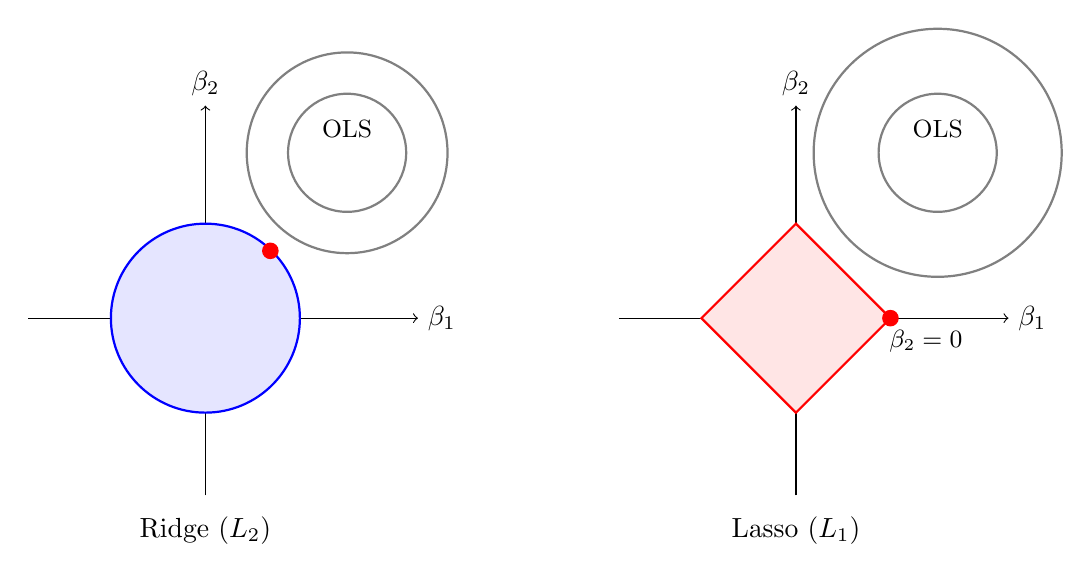
\begin{tikzpicture}[scale=1.5]
% Ridge (L2) - left plot
\begin{scope}[shift={(-2.5,0)}]
\draw[->] (-1.5,0) -- (1.8,0) node[right] {$\beta_1$};
\draw[->] (0,-1.5) -- (0,1.8) node[above] {$\beta_2$};
\draw[thick, blue, fill=blue!10] (0,0) circle (0.8);
\draw[thick, gray] (1.2,1.4) circle (0.5);
\draw[thick, gray] (1.2,1.4) circle (0.85);
\fill[red] (0.55,0.57) circle (2pt);
\node at (1.2,1.6) {\small OLS};
\node at (0,-1.8) {Ridge ($L_2$)};
\end{scope}

% Lasso (L1) - right plot
\begin{scope}[shift={(2.5,0)}]
\draw[->] (-1.5,0) -- (1.8,0) node[right] {$\beta_1$};
\draw[->] (0,-1.5) -- (0,1.8) node[above] {$\beta_2$};
\draw[thick, red, fill=red!10] (0.8,0) -- (0,0.8) -- (-0.8,0) -- (0,-0.8) -- cycle;
\draw[thick, gray] (1.2,1.4) circle (0.5);
\draw[thick, gray] (1.2,1.4) circle (1.05);
\fill[red] (0.8,0) circle (2pt);
\node at (1.2,1.6) {\small OLS};
\node at (1.1,-0.2) {\small $\beta_2 = 0$};
\node at (0,-1.8) {Lasso ($L_1$)};
\end{scope}
\end{tikzpicture}
\end{center}

The Lasso solution lands at a corner where $\beta_2 = 0$, demonstrating automatic variable selection.
\end{intuition}

\begin{bluebox}[Ridge vs Lasso: Summary]
\begin{center}
\begin{tabular}{lcc}
\toprule
\textbf{Property} & \textbf{Ridge ($L_2$)} & \textbf{Lasso ($L_1$)} \\
\midrule
Penalty & $\lambda \sum_j \beta_j^2$ & $\lambda \sum_j |\beta_j|$ \\
Closed-form solution & Yes & No \\
Shrinks coefficients & To small values & To exactly zero \\
Variable selection & No & Yes \\
Handles multicollinearity & Well & Arbitrarily selects one \\
Good when & Many small effects & Few large effects \\
\bottomrule
\end{tabular}
\end{center}
\end{bluebox}

\subsection{Elastic Net ($L_1$ + $L_2$ Penalty)}

\begin{definition}[Elastic Net]
\label{def:elastic-net}
\textbf{Elastic Net} combines the $L_1$ and $L_2$ penalties:
\begin{equation}
\min_{\boldsymbol{\beta}} \left\{ (\mathbf{y} - \mathbf{X}\boldsymbol{\beta})^\top (\mathbf{y} - \mathbf{X}\boldsymbol{\beta}) + \lambda_1 \sum_{j=1}^{p} |\beta_j| + \lambda_2 \sum_{j=1}^{p} \beta_j^2 \right\}
\label{eq:elastic-net-objective}
\end{equation}

Equivalently, with a single $\lambda$ and mixing parameter $\alpha \in [0, 1]$:
\begin{equation}
\min_{\boldsymbol{\beta}} \left\{ \text{SSE} + \lambda \left( \alpha \|\boldsymbol{\beta}\|_1 + (1 - \alpha) \|\boldsymbol{\beta}\|_2^2 \right) \right\}
\label{eq:elastic-net-alpha}
\end{equation}
where $\alpha = 1$ gives Lasso, $\alpha = 0$ gives Ridge, and intermediate values give a blend.
\end{definition}

\begin{intuition}[Why Elastic Net?]
Elastic Net addresses limitations of Lasso:
\begin{itemize}
    \item \textbf{Grouped selection:} When predictors are highly correlated, Lasso tends to select one arbitrarily and ignore others. Elastic Net tends to select groups of correlated variables together.
    \item \textbf{Stability:} The $L_2$ component stabilises the solution when $p > n$.
    \item \textbf{Flexibility:} The mixing parameter $\alpha$ allows tuning the balance between sparsity (Lasso-like) and grouping (Ridge-like).
\end{itemize}
\end{intuition}

\subsection{Choosing the Regularisation Parameter}

The regularisation parameter $\lambda$ (and $\alpha$ for Elastic Net) must be chosen carefully:
\begin{itemize}
    \item \textbf{Too small $\lambda$:} Minimal regularisation, overfitting risk.
    \item \textbf{Too large $\lambda$:} Excessive shrinkage, underfitting risk.
\end{itemize}

The standard approach is \textbf{cross-validation}:
\begin{enumerate}
    \item Split data into $k$ folds (typically $k = 5$ or 10).
    \item For each candidate $\lambda$, train on $k - 1$ folds and evaluate on the held-out fold.
    \item Repeat for all folds and average the prediction error.
    \item Select the $\lambda$ with lowest cross-validated error (or the largest $\lambda$ within one standard error of the minimum---the \emph{one-standard-error rule}).
\end{enumerate}

% =============================================================================
\section{Summary and Connections}
\label{sec:week8-summary}
% =============================================================================

\begin{keyresult}[Week 8 Key Results]
\textbf{Data structures:}
\begin{itemize}
    \item Scalar ($\mathbb{R}$), Vector ($\mathbb{R}^n$), Matrix ($\mathbb{R}^{m \times n}$), Tensor (higher-order arrays)
\end{itemize}

\textbf{Matrix operations:}
\begin{itemize}
    \item Transpose: $(\mathbf{A}\mathbf{B})^\top = \mathbf{B}^\top \mathbf{A}^\top$
    \item Multiplication: $(m \times n)(n \times p) = (m \times p)$; inner dimensions must match
\end{itemize}

\textbf{Linear systems:} $\mathbf{A}\mathbf{x} = \mathbf{b}$ solved via Gaussian elimination

\textbf{OLS estimator:}
\[
\hat{\boldsymbol{\beta}}_{\text{OLS}} = (\mathbf{X}^\top \mathbf{X})^{-1} \mathbf{X}^\top \mathbf{y}
\]

\textbf{Ridge estimator:}
\[
\hat{\boldsymbol{\beta}}_{\text{Ridge}} = (\mathbf{X}^\top \mathbf{X} + \lambda\mathbf{I})^{-1} \mathbf{X}^\top \mathbf{y}
\]

\textbf{Lasso:} No closed form; promotes sparsity via $L_1$ penalty
\end{keyresult}
